\chapter{Zeitlicher Arbeitsablauf}
\label{cha:Arbeit}
Dieses Kapitel spiegelt den chronologischen Ablauf des Projektes wieder und zeigt die Schritte auf, die notwendig waren um den Mikrocontroller so zu programmieren, dass dieser die Kommunikation zwischen RapidForm2004 und der vorhandenen Schrittmotorkarte ermöglicht. So das er sozusagen als Übersetzer für die unterschiedlichen Befehlssätze von RapidForm2004 und dem der Schrittmotorkarte fungiert.
%\begin{Tipp}
Die Codelistings in diesem Kapitel sind thematisch zusammen gefasst und gekürzt um die Lesbarkeit und das Verständnis zu gewährleisten. Ein komplettes Codelisting des Hauptprogramms befindet sich im Anhang \ref{sec:main.c}. Der komplette Code, mit allen Bibliotheken, liegt dem Praxisbericht als CD oder Archiv bei.
%\end{Tipp}
Kapitel \ref{sec:Erste_Schritte} beschreibt die Programmierung des Mikrocontrollers, welche die notwendigen Grundvoraussetzungen für dieses Projekt schafft. Das Ziel dieser Programmierung besteht darin die geforderten Komponenten, LEDs, LC-Display, Taster und serielle Schnittstellen im Mikrocontroller nutzbar zu machen.\\
Kapitel \ref{sec:Protokolle} beschreibt die Erarbeitung der Befehlssätze die die Software RapidForm2004 enthält um mit den von ihr unterstützten Schrittmotorkarten zu kommunizieren. Auch der Befehlssatz zur Kommunikation zwischen dem Mikrocontroller und der Schrittmotorkarte wird beschrieben.\\
Kapitel \ref{sec:Komm_SM} beschreibt wie der Mikrocontroller diesen Befehlssatz für die Kommunikation mit der vorhandenen Schrittmotorkarte nutzt.\\
Kapitel \ref{sec:Verbesserung_Hardware} gibt die Schritte zur Entwicklung und Verbesserung der Hardware, um diese so zu erweitern, dass sie den Vorgaben entspricht, wieder.\\
Kapitel \ref{sec:Komm_RF2004} erläutert die Kommunikation zwischen dem Mikrocontroller und RapidForm2004. \\
Kapitel \ref{sec:Auswerten_RF} beschreibt, wie die vorherigen Kapitel zusammenspielen, sodass eine reibungslose Kommunikation zwischen RapidForm2004 und der vorhandenen Schrittmotorkarte möglich ist.\\
Kapitel \ref{sec:Platinenlayout} beschreibt dann das Erstellen des Platinenlayouts und das Fertigen des Einschubs.

\section{Bereitstellen grundlegender Funktionalitäten}
\label{sec:Erste_Schritte}
Im ersten Schritt ging es darum, den Mikrocontroller so zu programmieren, dass dieser die für dieses Projekt grundlegenden Funktionalitäten bereitstellen kann.\\
Der Mikrocontroller befand sich vorerst auf dem \Fachbegriff{STK500}(siehe Kapitel \ref{sec:STK500}). Um dessen Komponenten im Mikrocontroller nutzen zu können, müssen dafür Register initialisiert werden oder Funktionalitäten wie z.B. Bibliotheken für das LC-Display bereit gestellt werden.\\
Die folgenden Kapitel beschreiben den Programmcode, der notwendig ist um diese Funktionalitäten bereitzustellen.
\subsection{Taster}
\label{sec:Taster}
Um die Taster des STK500 im Mikrocontroller nutzen zu können müssen diese mit dem Mikrocontroller verbunden und entprellt\footnote{Als \Fachbegriff{Prellen} bezeichnet man das ungewollte mehrfache Schalten eines mechanischen Schalters bei einem einzelnen Schaltvorgang.} werden.\\
Dazu muss die Stiftleiste von \emph{PortA} mit der Stiftleiste für die Taster verbunden werden. Das Entprellen der Taster wird softwareseitig realisiert. Dies bietet sich bei einem Mikrocontroler an. Dazu gibt es vorgefertigte Bibliotheken die genutzt werden können. Im Projekt wurde die Bibliothek \Datei{Debounce.h}\cite{uC:Dannegger} von Peter Dannegger genutzt. Sie ist sehr komfortabl und funktionsreich und basiert auf \Fachbegriff{Timer-Interrupts}. Um sie zu nutzen wird die Datei \Datei{Debounce.h} in das Projektverzeichnis kopiert und mit Zeile 1 des Codelisting \ref{lst:Taster} in das Programm eingebunden. Die Zeilen 2-10 spiegeln die Funktion zum Initialisieren der Bibliothek wieder. Diese Zeilen müssen auf den jeweils verwendeten Mikrocontroller angepasst werden.\\
Durch die Verwendung der Bibliothek ist es möglich Funktionen wie z.B. \linebreak \Code{get\_key\_press()} zu nutzen um den Status der Taster prellfrei auszulesen und diese Information für Entscheidungen im Programmablauf zu verwenden. 
\lstset{language=C, basicstyle=\footnotesize, showstringspaces=false, tabsize=8}
\lstinputlisting[label=lst:Taster,caption=Taster]{Code/taster.c}

\subsection{LEDs}
\label{sec:LED}
LEDs sollen im Programmablauf genutzt werden können, um z.B. Fehler zu signalisieren.\\
Dazu muss zuerst die Stiftleiste von \emph{PortB} mit der LED Stiftleiste des STK500 verbunden werden. Um LEDs an \emph{PortB} betreiben zu können müssen die entsprechenden Pins im \Fachbegriff{Register} \Code{DDRB} als Ausgänge definiert werden. Dies geschieht in Zeile 1 des Codelisting \ref{lst:LED}. Die Bibliothek zum Entprellen der Taster nutzt die Variablen \Code{LED\_DDR} und \Code{LED\_PORT}. Diese Variablen werden auch hier genutzt um auf die Register zuzugreifen. Dies gewährleistet eine bessere Übersicht. Die Werte im 8-Bit Register \Code{LED\_PORT} spiegeln die Spannungen an den Pins des \emph{PortB} am Mikrocontroller wieder. Da die LEDs auf dem STK500 mit \Fachbegriff{active-low-Logik} betrieben werden, muss das jeweilige Bit gelöscht, also auf ''0'', gesetzt werden damit die LED leuchtet. Um alle Bits in einem Register zu verändern kann das Register mit einem 2-stelligen Hex-Wert (8-Bit) oder einem 8 stelligen binären Bitmuster beschrieben werden. In Zeile 2 werden alle Bits mit dem Hex-Wert \Code{0xFF} auf ''1'' gesetzt und somit alle LEDs ausgeschaltet. Um ein einzelnes Bit zu verändern, können die Anweisungen in den Zeilen 3 und 4 verwendet werden. Dabei steht das ''X'' in \emph{PBX} für die x-te Stelle im Register die gesetzt oder gelöscht werden soll.\\
Es ist damit möglich im Programmablauf einzelne LEDs anzusteuern.
\lstset{language=C, basicstyle=\footnotesize, showstringspaces=false, tabsize=8}
\lstinputlisting[label=lst:LED,caption=LEDs]{Code/led.c}

\subsection{Ansteuerung des LC-Display}
\label{sec:LCD}
Um den aktuellen Status des Motor komfortabel in Textform anzeigen zu können und die Schrittmotorkarte \emph{menübasiert} ansteuern zu können wird ein \Fachbegriff{LC-Display} verwendet. Das verwendete Display ist \Fachbegriff{alpha numerisch} und kann 4x20 Zeichen anzeigen.\\
Die meisten LC-Displays werden auf die gleiche Weise angesteuert. Hier gibt es fertige Bibliotheken die frei genutzt werden können. Im Projekt wurde die Bibliothek von Peter Fleury \cite{uC:Fleury} verwendet. Die Bibliothek wird heruntergeladen und die Dateien \Datei{lcd.c} und \Datei{lcd.h} in das Projektverzeichnis entpackt. Die Bibliothek wird mit \Code{\#include ''lcd.h''} eingebunden. In der \Datei{lcd.h} müssen dann noch die Daten des Displays eingegeben werden (siehe Codelisting \ref{lst:LCD} Zeilen 2--10).\\
Danach kann das Display im Programm mit den Befehlen aus Zeile 12--21 angesteuert werden.
\lstset{language=C, basicstyle=\footnotesize, showstringspaces=false, tabsize=8}
\lstinputlisting[label=lst:LCD, caption=lcd.h (Auszug)]{Code/lcd_def.c}

\subsection{RS-232-Schnittstelle}
\label{sec:RS232}	
\Fachbegriff{RS-232} ist der Name der am häufigsten verwendeten seriellen Schnittstelle um Daten zwischen zwei elektronischen Geräten hin und her zu senden. \cite{uC:RS232}\\
Auf dem STK500 ist bereits eine serielle Schnittstelle vorbereitet. Um diese nutzen zu können, müssen die Pins 3 und 4 des \emph{PortC} (erster \Fachbegriff{UART}) des Mikrocontrollers mit der Stiftleiste \emph{Rx/Tx} auf dem STK500 verbunden werden. Eine weitere Schnittstelle wurde auf einem Steckbrett aufgebaut. Diese wurde mit den Pins 1 und 2 des \emph{PortC} (zweiter UART) des Mikrocontrollers verbunden. Um die Schnittstellen im Mikrocontroller nutzen zu können müssen diese noch durch setzen von Bits in den entsprechenden Registern des Mikrocontrollers aktiviert werden.\\
Das Codelisting \ref{lst:RS232} teilt sich in 4 wesentliche Bereiche: \\
\begin{itemize}
\item Zeilen 1 -- 2: Setzen der Baudrate und einbinden der benötigten Bibliotheken.
\item Zeilen 3 -- 17: Initialisieren der Schnittstellen durch setzen der richtigen Bits in den entsprechenden Registern.
\item Zeilen 18 -- 35: Funktionen zum Senden von Daten
\item Zeilen 36 -- 65: Funktionen zum Empfangen von Daten
\end{itemize}
\lstset{language=C, basicstyle=\footnotesize, showstringspaces=false, tabsize=8}
\lstinputlisting[label=lst:RS232,caption=RS-232]{Code/rs232.c}
Damit stehen die essentiellen Funktionen \Code{uart\_put\_string(dir)} und \linebreak\Code{uart\_get\_string(dir)} zur Verfügung. Mit diesen kann der Mikrocontroller über die serielle Schnittstelle Strings senden und empfangen. Der Parameter \Code{dir} gibt dabei die Schnittstelle an über die gesendet oder empfangen werden soll.

\section{Befehlssätze} 
\label{sec:Protokolle}
Das zu erreichende Ziel bestand darin, dass RapidForm2004 mit dem Mikrocontroller und dieser mit der Schrittmotorkarte kommunizieren können sollte. Die Kommunikation läuft dabei über Befehle ab, die über die serielle Schnittstelle gesendet werden. 
%Die Befehlssätze die im Projekt verwendet werden um mit den Schrittmotorsteuerungen zu kommunizieren, werden als Protokolle bezeichnet. In diesen Protokollen ist geregelt, welche Befehle ausgesendet werden müssen und welche Antworten auf diese Befehle erwartet werden.\\
Jede Schrittmotorkarte verwendet eigenen Befehle. Alle Befehle für eine Schrittmotorkarte werden im Folgenden als Befehlssatz bezeichnet. Die Software RapidForm2004 kennt mehrere Befehlssätze um verschiedene Schrittmotorkarten anzusteuern. Der Befehlssatz der vorhandenen Schrittmotorkarten zum Ansteuern der Motoren des Drehtisches ist jedoch nicht in RapidForm2004 vorhanden.\\
Nun soll der Mikrocontroller sowohl mit RapidForm2004 als auch mit der ersten der vorhandenen Schrittmotorkarten kommunizieren. Befehle an die zweite Schrittmotorkarte werden über die Erste gesendet. Um mit beiden Seiten kommunizieren zu können muss der Mikrocontroller den Befehlssatz der vorhanden Schrittmotorkarten und zumindest einen der Befehlssätze aus RapidForm2004 kennen. Außerdem muss er wissen welche Antwort RapidForm2004 auf einen gesendeten Befehl erwartet. \\
In der ersten Phase wurde die Software \emph{Free Serial Port Monitor} verwendet um die Kommunikation zwischen RapidForm2004 und dem Mikrocontroller abzuhören. Dies hatte jedoch den Nachteil, das RapidForm2004 erst dann den nächsten Befehl sendete, wenn der Erste mit der erwarteten Antwort quittiert wurde. Die Befehle die RapidForm erwartete, konnten zwar teilweise aus den Betriebsanleitungen der Schrittmotorsteuerungen entnommen werden, dieses Vorgehen war jedoch sehr mühsam. Eine besseres Vorgehen, war das sogenannte \Fachbegriff{Reverse-Engineering}. Dadurch konnten alle Befehe und die darauf erwarteten Antworten aus einer ausführbaren Datei von RapidForm2004 ausgelesen werden.\\
Das Codelisting \ref{lst:Proto_RF_Isel} zeigt einen Auszug für den Befehlssatz eines Isel Schrittmotors. Im Anhang \ref{sec:Protokolle_RF} befinden sich die Befehlssätze aller Schrittmotorkarten. Somit stehen die Befehlssätze aller Schrittmotorsteuerungen zur Verfügung. Diese wurden in einer Textdatei gespeichert und werden später im Programm verwendet. Dadurch sind alle Befehle und die Antworten die RapidForm2004 auf einen daraus ausgesendeten Befehl erwartet bekannt.
%\begin{Tipp}
In Codelistings und im Quelltext wird teilweise noch die Bezeichnung \emph{Protokolle} statt \emph{Befehlssätze} verwendet. Diese sind gleichbedeutend.
%\end{Tipp}
\lstset{language=C, basicstyle=\footnotesize, showstringspaces=false, tabsize=8}
\lstinputlisting[label=lst:Proto_RF_Isel,caption=Befehlssatz aus Rapidform: Isel]{Code/Protokolle_RF_Isel.txt}

\section{Kommunikation mit der vorhandenen Schrittmotorsteuerung}
\label{sec:Komm_SM}
\subsection{Befehle senden}
\label{sec:menu}
Im nächsten Schritt geht es darum, Befehle an die Schrittmotorkarte zu versenden. Da es nicht möglich ist, für jeden Befehl eine eigene Taste zu verwenden, 
wird eine menübasierte Steuerung mittels des LC-Displays verwendet. Im Menü lässt sich mit den Tasten \emph{Hoch}, \emph{Runter}, \emph{Ok}, und \emph{Zurück}, navigieren.\\
Analog wie beim LC-Display und bei den Tastern wird hier eine vorhandene Bibliothek genutzt. Um die Bibliothek verwenden zu können musste die Menüstruktur den Bedürfnissen des Projekts angepasst werden und die Funktionen zum Ausgeben von Text auf dem LC-Display und zum Versenden von Befehlen über die RS-232-Schnittstelle, aus den vorangegangen Kapiteln, bekannt gemacht werden. Dies geschieht in der Datei \Datei{tinymenu/tinymenu.h}.\\
Die Zeilen 1--6 des Codelisting \ref{lst:Menu} dienen zum Einbinden der benötigten Bibliotheken. Die Zeilen 8--20 zeigen eine vereinfachte Struktur des Hauptprogramms. Wird ein Taster gedrückt, wird dies durch die \Code{get\_key\_press()}-Funktion, bekannt aus Kapitel \ref{sec:Taster}, erkannt und die entsprechende Menü Funktion aufgerufen.
\lstset{language=C, basicstyle=\footnotesize, showstringspaces=false, tabsize=8}
\lstinputlisting[label=lst:Menu,caption=Menü]{Code/menu.c}
Folgende Menüpunkte wurden realisiert:
\lstset{language=C, basicstyle=\footnotesize, showstringspaces=false, tabsize=8}
\lstinputlisting[label=lst:Menu_Baum,caption=Menü Baum]{Code/menu_main.txt}
Wird einer der Menüpunkte aufgerufen, wird die im Menüpunkt hinterlegte Funktion mit dem hinterlegten Parameter aufgerufen. Wird beispielsweise der Befehl \emph{+90} ausgewählt, wird die hinterlegte Funktion \Code{menu\_puts(arg, name)}(Codelisting \ref{lst:Menu} Zeile 18-28) mit dem hinterlegten Wert aufgerufen. Diese sendet dann mit der aus Kapitel \ref{sec:RS232} bekannten Funktion \Code{uart\_puts(arg, dir)} einen Befehl an die Schrittmotorsteuerung.\\
Es ist somit nun möglich mit Tastern vordefinierte Befehle aus dem Menü auszuwählen und an die Schrittmotorsteuerung zu senden.
\subsection{Antworten empfangen und speichern}
\label{sec:Empfangen_Schrittmotor}
Die Schrittmotorsteuerung antwortet auf Befehle mit einem \Fachbegriff{String}. In diesem Arbeitsschritt wird die Funktionalität zum Empfangen von Antworten der Schrittmotorsteuerung auf Befehle des Mikrocontrollers hergestellt. Diese Antworten sollen in einem String gespeichert und im nächsten Schritt an eine \emph{Auswerte-Funktion} weiter gegeben werden.\\
Dazu wird in der Hauptschleife des Programms ständig das Eingangsregister der ersten seriellen Schnittstelle abgefragt (siehe Codelisting \ref{lst:rs232empfangstepper} Zeile 10--13). Dieses Vorgehen bezeichnet man als \Fachbegriff{Polling}.
Sind Daten im Register vorhanden, wird \Code{LED3} eingeschaltet und die Funktion \Code{uart\_rx(int dir)} mit dem Parameter \Code{D\_Stepper} aufgerufen. Der übergebene Parameter gibt an, dass der Befehl von der für die Schrittmotorkarte zuständigen Schnittstelle empfangen wurde. Dadurch wird sichergestellt, dass der empfangene \Fachbegriff{String} aus dem richtigen Datenempfangsregister ausgelesen wird und festgelegt wie er weiterverarbeitet wird. Die Funktion \Code{uart\_rx(dir)} liest dann das Empfangsregister mit der aus Kapitel \ref{sec:RS232} bekannten Funktion \linebreak\Code{uart\_get\_string(str\_rx, dir)} aus und schreibt den empfangenen String in die Variable \Code{str\_rx}(Codelisting \ref{lst:rs232empfangstepper}, Zeile 7). In einer \Fachbegriff{if-Abfrage} wird entschieden von welcher Schnittstelle der empfangene Befehl kam. Da \Code{D\_Stepper} übergeben wurde, wird der if-Teil der Abfrage ausgeführt. In dieser wird der empfangene String an die \emph{Auswerte-Funktion} für die Schrittmotorkarte (Codelisting \ref{lst:rs232empfangstepper}, Zeile 15-45) übergeben.
Durch diesen Teil des Programms ist es nun möglich Antworten der Schrittmotorkarte zu empfangen, in dem String \Code{str\_rx} zu speichern und an die Auswerte-Funktion \Code{switch\_Stepper(str\_rx)} zu übergeben.
\lstset{language=C, basicstyle=\footnotesize, showstringspaces=false, tabsize=8}
\lstinputlisting[label=lst:rs232empfangstepper, caption=RS-232 Empfang]{Code/rs232_empfang_stepper.c}


\subsection{Antworten auswerten}
\label{sec:Auswerten_SM}
Die Funktion zum Auswerten empfangener Strings spielt eine zentrale Rolle im Projekt. Diese Funktion ermöglicht es, ankommende Strings im Mikrocontroller gegen die bekannten Antworten zu prüfen und eine entsprechende Reaktion auszuführen.\\
In der Auswerte-Funktion wird der übergebene String mittels der Funktion\\
\Code{FindStringInArray(str\_rx, pOptions, length)}(Codelisting \ref{lst:FindString}) gegen ein \Fachbegriff{Array} (Codelisting \ref{lst:switchStepper}, Zeile 3) mit bekannten Befehlen geprüft. Ist der String in diesem Array vorhanden, wird die Position des Strings im Array zurückgegeben, ansonsten wird ''99'' zurückgegeben. In einer anschließenden \Fachbegriff{switch/case-Struktur} wird dann der Position im Array ein bestimmtes Verhalten des Mikrocontrollers zugeordnet. Wird beispielsweise der String \Code{\#} empfangen, wird Position \Code{0} zurück gegeben und auf dem LC-Display wird \emph{Erfolgreich} ausgegeben.\\
Durch diese Funktion kann nun auf Strings reagiert werden und eine entsprechende Reaktion seitens des Mikrocontrollers erfolgen. 
\lstset{language=Java, basicstyle=\footnotesize, showstringspaces=false, tabsize=8}
\lstinputlisting[label=lst:FindString, caption=FindStringInArray()]{Code/FindString.c}
\lstset{language=Java, basicstyle=\footnotesize, showstringspaces=false, tabsize=8}
\lstinputlisting[label=lst:switchStepper, caption=switchStepper()]{Code/switch_stepper.c}

\section{Verbesserungen an der vorhandenen Hardware}
\label{sec:Verbesserung_Hardware}
\subsection{Netzteil}
\label{sec:Netzteil}
Ziel dieses Arbeitsschrittes war es, die festen Lötverbindungen zwischen dem PC-Netzteil und den einzelnen Karteneinschüben im 19''-Rack durch Steckverbindungen zu ersetzen und dadurch leicht erweiterbar zu machen.\\
Die festen Lötverbindungen am Einschub für die Schrittmotorkarte wurden durch Standard PC-Netzteil Stecker ersetzt. %Die Mikrocontroller-Platine wird mit \emph{5V} gespeist.
Die \Fachbegriff{Logikbausteine} der Schrittmotorkarte werden mit \emph{5V} gespeist. Die Schrittmotorkarte wird zusätzlich mit \emph{12V} für den Schrittmotor gespeist. Der Stecker lässt sich nun einfach mit einer Buchse des Standard PC-Netzteils verbinden und es ist nicht mehr Notwendig zu löten wenn das Netzteil ausgebaut wird. Mittels eines Y-Kabels(siehe Abbildung \ref{fig:Y-Kabel}) können nun leicht weitere Buchsen hinzugefügt werden.\\
Dadurch kann das Netzteil nun einfach ein- und ausgebaut werden, bzw. das System leicht um neue Einschubkarten erweitert werden.
\begin{figure}[h]
\centering
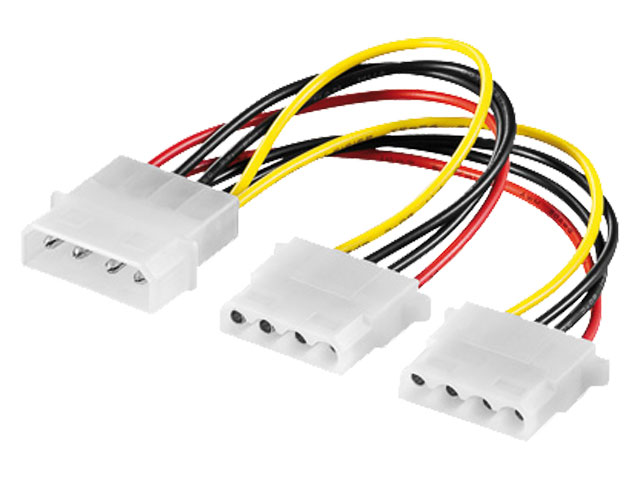
\includegraphics[width=100pt]{Y-Kabel.jpg}
\caption{Stromverbinder - Y-Kabel\cite{kosatec}}
\label{fig:Y-Kabel}
\end{figure}

\subsection{Zweite Schrittmotorkarte}
Zu Anfang war nur eine Schrittmotorkarte für die Rotation des Drehtisches vorbereitet. Mit einem zweiten Schrittmotor konnte der Tisch in der Höhe verstellt werden. Für diesen fehlte jedoch noch eine zweite Schrittmotorkarte. Diese musste noch vorbereitet und mit der Ersten verbunden werden.\\
Dazu wurde, wie in Kapitel \ref{sec:Netzteil} beschrieben, ein weiterer Einschubplatz für die Schrittmotorkarte vorbereitet. Die Karte wurde mit einer Frontblende versehen und auf dieser eine Buchse für die Motorverkabelung und je eine Buchse und einen Stecker für die seriellen Schnittstellen verbaut. Diese wurden mit den entsprechenden Anschlüssen auf der Schrittmotorkarte verlötet. Die Karte wird in den Einschubplatz geschoben und mit einem seriellen Kabel als \Fachbegriff{Daisy-Chain} mit der ersten Schrittmotorkarte verbunden. Dadurch kann die zweite Schrittmotorkarte über die Erste angesteuert werden.\\
Somit steht eine baugleiche Schrittmotorkarte zur Verfügung. Diese kann nun den Schrittmotor für die Höhenverstellung ansteuern. Befehle an diese Schrittmotorkarte werden an die erste Karte geschickt, jedoch mit dem Prefix \emph{2}. Dieser weist die erste Karte an, den Befehl an die zweite Karte weiter zu senden. So kann das System um weitere Karten erweitert werden.

\subsection{Motor- und Endschalterverkabelung}
Zwischen der zweiten Schrittmotorkarte und dem zugehörigen Schrittmotor, der für die Höhenverstellung zuständig ist, war noch kein Kabel vorhanden. Dieses musste noch gefertigt und um 3 Leitungen für die Endschalter erweitert werden.\\
Dafür wurde in der Werkstatt des RheinAhrCampus Remagen ein 7 adriges Kabel (siehe Abbildung \ref{fig:Motorverkabelung}) besorgt und die passenden Endstecker bestellt. Die Belegung wurde gleich zum Kabel für den ersten Schrittmotor gewählt, jedoch um die 3 Adern für die beiden Endschalter erweitert. Tabelle \ref{tab:Motorverkabelung} gibt die Belegung des Kabels wieder.\\
Somit stand ein Kabel zur Verfügung mit dem sowohl der Schrittmotor gesteuert, als auch der Status der Endschalter an die Schrittmotorkarte übermittelt werden konnte.
\begin{figure}[h]
\centering
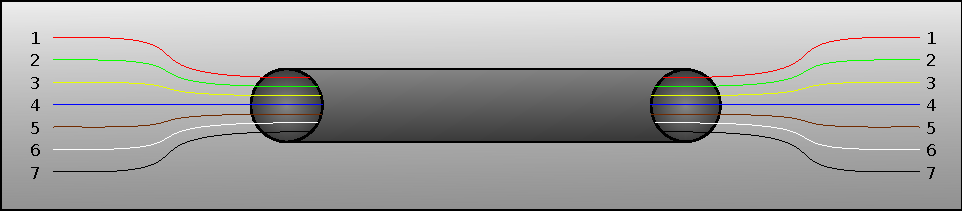
\includegraphics[width=\textwidth]{Kabel.pdf}
\caption{Motor- und Endschalterverkabelung}
\label{fig:Motorverkabelung}
\end{figure}


\begin{longtable}{|c|l|} 
\caption{Motor- und Endschalterverkabelung}\\
\hline
\label{tab:Motorverkabelung}1 & Phase A\\ \hline 
2 & Phase B\\ \hline 
3 & Phase C\\ \hline 
4 & Phase D\\ \hline 
5 & Endschalter oben\\ \hline 
6 & Endschalter unten\\ \hline 
7 & Endschalter Masse\\ \hline 
\end{longtable} 
\subsection{Endschalter}
Nun sollen die vorgegeben induktiven Endschalter mit der Schrittmotorkarte und dem Mikrocontroller zu verbinden. Dadurch soll gewährleistet werden, dass der Drehtisch nicht über den Arbeitsbereich hinaus bewegt werden kann. Zusätzlich soll das Erreichen der Endpositionen auf dem LC-Display angezeigt werden.\\
Da die Schrittmotorkarte nur mechanische Endschalter unterstützt, ließen sich die induktiven Endschalter nicht ohne weiteres nutzen. Um die induktiven Endschalter nutzen zu können, musste die Spannung über einen Spannungsteiler heruntergesetzt werden und die standardmäßigen Eingänge für die mechanischen Endschalter umgangen werden. Die induktiven Endschalter werden direkt an den Optokoppler angeschlossen, welcher für die mechanischen Endschalter zuständig ist. Dadurch wurden die Signale der Endschalter für die Schrittmotorkarte nutzbar.
\begin{figure}[h]
\centering
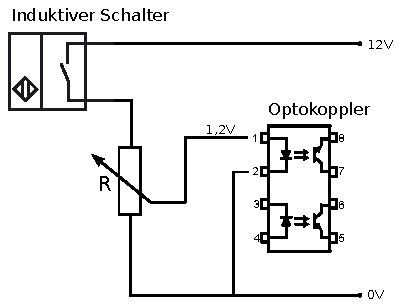
\includegraphics{Endschalter.pdf}
\caption{Endschalterverkabelung}
\label{fig:Endschalterverkabelung}
\end{figure}
Ein weiteres Problem bestand darin, dass, wenn der Tisch sich bereits in der Endposition befand, die Endschalter noch nicht aktiviert wurden. Dies lag daran, dass der Metallstutzen, der die Endschalter auslösen sollte, sich nicht im Schaltbereich der induktiven Schalter befand. Zur Abhilfe wurde ein längerer Metallstutzen von der Werkstatt des RheinAhrCampus angefertigt.\\
Wenn der Tisch sich in der Endposition befindet, soll dies auch auf dem LC-Display angezeigt werden. Die Signale der Endschalter liegen auf der Rückseite der Schrittmotorkarte am Verbindungsstecker an. Um die Signale dem Mikrocontroller zugänglich zu machen wurde eine Brücke zwischen den Verbindungssteckern der Schrittmotorkarte und der Mikrocontroller-Platine gelötet. Auf der Mikrocontroller-Platine sind diese beiden Pins mit je einem Pin des Mikrocontrollers verbunden. Diese beiden Pins werden im Mikrocontroller als \Fachbegriff{Interrupts} definiert. Die \Fachbegriff{Interrupt-Service-Routine} zum Anzeigen der Nachricht auf dem LC-Display wird in Kapitel \ref{sec:Endschalter_SW} beschrieben.\\
Da die Signale der Endschalter nun an der Schrittmotorkarte anliegen, stoppt diese den Motor wenn eine der Endschalterpositionen erreicht wird. Zusätzlich liegen die Signale am Mikrocontroller an. Dieser gibt dadurch auf dem Display die Meldung \emph{Endschalterposition erreicht!} aus.

\subsection{Zweite serielle Schnittstelle}
Das STK500 bietet nur eine serielle Schnittstelle. Um zusätzlich zur Schrittmotorkarte auch mit RapidForm2004 kommunizieren zu können, wird eine zweite RS-232-Schnittstelle benötigt.\\
Dafür wurde vorerst auf einem Steckbrett eine zweite serielle Schnittstelle nach dem Schaltplan in Abbildung \ref{fig:MAX232} aufgebaut. Später wird diese Schnittstelle direkt auf der Mikrocontroller-Platine realisiert.
Dadurch ist es möglich mit dem Mikrocontroller über zwei RS-232-Schnittstellen gleichzeitig zu kommunizieren.
\begin{figure}[h]
\centering
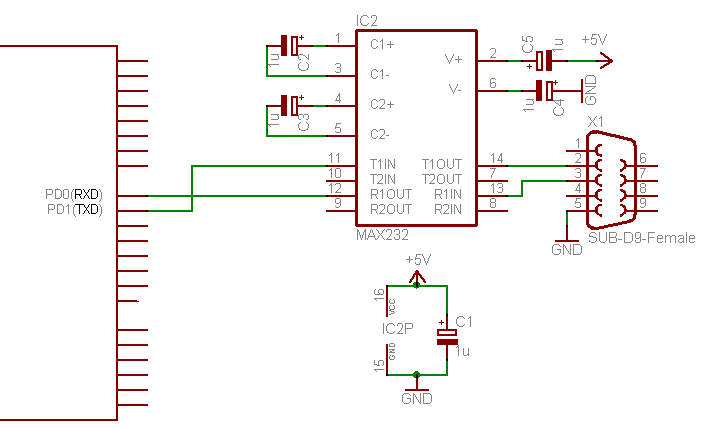
\includegraphics[width=0.6\textwidth]{AVR-RS232}
\caption{Schaltplan für die zweite serielle Schnittstelle
\cite{uC:RS232}}
\label{fig:MAX232}
\end{figure}

\section{Kommunikation mit RapidForm2004}
\label{sec:Komm_RF2004}
RapidForm2004 sendet Befehle die für die Drehtischsteuerung bestimmt sind an den Mikrocontroller. Diese sollen dort empfangen, ausgewertet und in verständlicher Form an die Drehtischsteuerung weiter gegeben werden. RapidForm2004 verwendet dabei verschiedene Befehlssätze für verschiedene Schrittmotorsteuerungen. Für jeden dieser Befehlssätze wird eine eigene Auswerte-Funktion geschrieben. Im folgenden Kapitel wird nun das Empfangen der Befehle beschrieben und eine erste Auswertung, die den empfangenen Befehl dem Befehlssatz einer Schrittmotorsteuerung zuordnet. 
Nachdem ein Befehl zugeordnet wurde und in der entsprechenden Auswerte-Funktion erkannt wurde, soll ein entsprechender Befehl an die Drehtischsteuerung gesendet und die Antwort der Drehtischsteuerung vom Mikrocontroller ausgewertet werden. Abschließend soll eine entsprechende Antwort an RapidForm2004 zurück gesendet werden. Abbildung \ref{fig:Schema_Komm} zeigt eine schematische Übersicht dieser Kommunikation.\\
Die Kommunikation mit RapidForm2004 ist ähnlich zu der mit der Schrittmotorsteuerung. Diese wurde bereits in Kapitel \ref{sec:Komm_SM} ausführlich beschrieben. Daher wird die Kommunikation hier etwas oberflächlicher behandelt.
\begin{figure}[h]
\centering
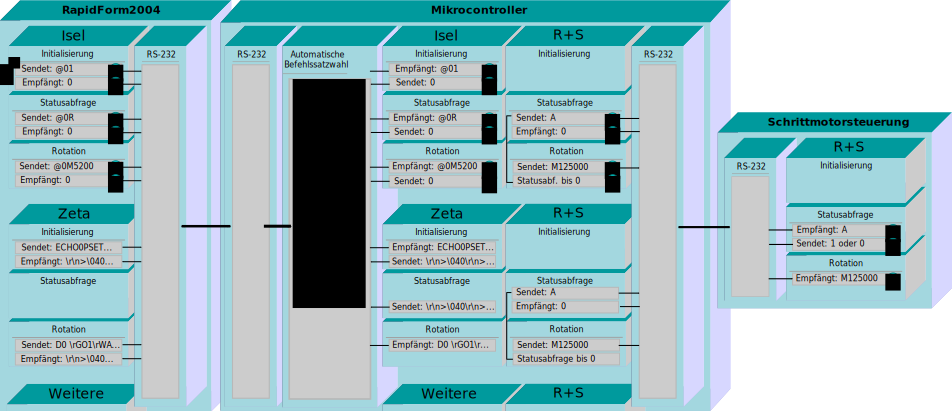
\includegraphics[width=\textwidth]{Schema_Kommunikation}
\caption{Schema der Kommunikation}
\label{fig:Schema_Komm}
\end{figure}

\subsection{Befehle empfangen}
Zuerst sollen nun die Befehle von RapidForm2004 an den Mikrocontroller, gespeichert werden. Anschließend wird die automatische Auswahl des Befehlssatzes beschrieben.\\
Um anstehende Befehle zu empfangen wird, ähnlich wie in Kapitel \ref{sec:Empfangen_Schrittmotor}, eine Funktion die ständig das Eingangsregister der ersten seriellen Schnittstelle abfragt verwendet (siehe Codelisting \ref{lst:rs232empfangrf}). Auch hier wird die Funktion \Code{uart\_rx(dir)} aufgerufen, jedoch mit dem Parameter \Code{D\_RapidForm}. Der empfangenen String wird auch hier in die Variable \Code{str\_rx} gespeichert. Somit können nun auch Strings von RapidForm2004 empfangen und in der Variablen \Code{str\_rx} gespeichert werden.
\lstset{language=Java, basicstyle=\footnotesize, showstringspaces=false, tabsize=8}
\lstinputlisting[label=lst:rs232empfangrf, caption=RS-232 Empfang - RapidForm2004]{Code/rs232_empfang.c}

\subsubsection{Automatische Auswahl eines Befehlssatzes}
\label{sec:AutoProtokoll}
Nun geht es darum, dass der Mikrocontroller anhand eines ersten Befehls der empfangen wird, festlegt, mit welchem Befehlssatz fortan kommuniziert werden soll. Die Kennung für den Befehlssatz wird in einer globalen Variable gespeichert und alle weiteren Befehle werden an die entsprechende Auswerte-Funktion für diesen Befehlssatz übergeben.\\
In der Funktion \Code{uart\_rx(dir)}(Codelisting \ref{lst:uartrx}) wird nun in der ersten \emph{if-Abfrage} entschieden, von welcher Schnittstelle der empfangene Befehl kam. Diese verzweigt nun, da \Code{D\_RapidForm} übergeben wurde, in den else-Teil. In diesem wird mit mehreren \emph{if-Abfragen} überprüft, ob bereits der Befehlssatz für einen bestimmten Motor ausgewählt wurde. Ist dies nicht der Fall, wird der empfangende String an die Funktion \Code{switch\_Motor(str\_rx)}(Codelisting \ref{lst:switchMotor}) übergeben. Diese prüfte mit der aus Kapitel \ref{sec:Auswerten_SM} bekannten Funktion \Code{FindStringInArray(str\_rx, pOptions, 3)}, den angekommenen String gegen die Initialisierungsbefehle der einzelnen Befehlssätze. Die Initialisierungsbefehle sind die ersten Befehle die RapidForm2004 an eine Schrittmotorsteuerung sendet um zu prüfen ob diese vorhanden ist. In diesem ersten Schritt wird der String nur zur Identifizierung des von RapidForm2004 verwendeten Befehlssatzes verwendet. Das Antworten auf einen String wird erst in den nachfolgenden Kapiteln beschrieben. Die Funktion \Code{switch\_Motor(str\_rx)} gibt einen numerischen Wert zurück. Jede Zahl entspricht dabei dem Befehlssatz für eine Schrittmotorsteuerung. Die Zahlenwerte werden dabei mittels Makro-Definitionen (Codelisting \ref{lst:switchMotor} Zeile 1-6) durch lesbare Text-Variablen ersetzt. Dies erhöhte die Lesbarkeit und das Verständnis. War dieser Schritt erfolgreich, wird in den folgenden if-Abfragen die richtige Auswerte-Funktion aufgerufen. Konnte die Funktion \Code{switch\_Motor(str\_rx)} den empfangen Befehl nicht zuordnen, gibt sie \Code{M\_UNK} zurück und es wird auf dem Display \emph{Unbekannter Motor!} ausgegeben.\\
Somit ist es möglich Befehle von RapidForm2004 zu empfangen und an die richtige Auswerte-Funktionen zu übergeben. Zusätzlich wird die Programmierung dadurch wesentlich robuster, da unbekannte Befehle ignoriert werden.\\
Der Nachteil dieses Vorgehens besteht darin, dass für ein wechseln des Befehlssatzes der Mikrocontroller neu gestartet werden muss. Ein Beheben dieses Nachteils wäre nicht ohne weiteres möglich gewesen.

\lstset{language=C, basicstyle=\footnotesize, showstringspaces=false, tabsize=8}
\lstinputlisting[label=lst:uartrx,caption=Funktion: uart rx()]{Code/uart_rx.c}

\lstset{language=C, basicstyle=\footnotesize, showstringspaces=false, tabsize=8}
\lstinputlisting[label=lst:switchMotor,caption=Funktion: switch Motor()]{Code/switch_Motor.c}

\section{Auswerte-Funktionen}
\label{sec:Auswerten_RF}
Die Auswerte-Funktionen sind das Herzstück des Programms. Es geht darum für jedes Protokoll eine eigene Auswerte-Funktion zu schreiben. Diese sollen die von RapidForm2004 kommenden Strings verstehen können und in einen, für die vorhandene Schrittmotorkarte, verständlichen Befehl übersetzen können. Die Funktionen sollen weiterhin prüfen, ob der Befehl von der Schrittmotorkarte erkannt wurde und den Status der Schrittmotorkarte zurück an RapidForm2004 melden.\\
Alle bisherigen Arbeitsschritte hatten zum Ziel, die Kommunikation zwischen RapidForm2004 und der ersten Schrittmotorkarte zu ermöglichen. Nun fehlt nur noch der Teil des Programms der die ankommenden Befehle auswertet und in verständlicher Form an die Schrittmotorkarte weitergibt.
Im folgenden Kapitel wird dieser Ablauf nun exemplarisch für den Befehlssatz eines Isel-Motors erklärt.

\subsection{Auswerte-Funktion für Isel-Motoren}
Wird der Befehl \Code{@01} empfangen, übergibt die in Kapitel \ref{sec:AutoProtokoll} beschriebene Funktion, den String an die Auswerte-Funktion \Code{switch\_Isel(str\_rx)}. Der Ablauf dieser Funktion ist ähnlich aufgebaut wie bei der Kommunikation mit der Schrittmotorkarte (Kapitel \ref{sec:Komm_SM}) und bei der automatischen Auswahl des Befehlssatzes (Kapitel \ref{sec:AutoProtokoll}. In der Funktion \Code{switch\_Isel(str\_rx)} sind in dem Array \Code{pOptions} alle benötigten Befehle des Isel-Befehlssatzes hinterlegt. Mit der aus Kapitel \ref{sec:Auswerten_SM} bekannten Funktion \Code{FindStringInArray(str\_rx, pOptions)} wird  \Code{str\_rx} gegen diese Befehle geprüft. Wird der Befehl im Array gefunden gibt die Funktion \Code{FindStringInArray()} die Position des Strings im Array zurück. Mittels einer \Fachbegriff{switch-case-Struktur} lässt sich nun so für jeden Befehl ein entsprechender Ablauf ausführen. Die einzelnen Abläufe werden übersichtlich in den folgenden Kapiteln beschrieben.
\lstset{language=C, basicstyle=\footnotesize, showstringspaces=false, tabsize=8}
\lstinputlisting[label=lst:switch_Isel,caption=Übersetzungs Logik für einen Isel-Motor]{Code/switch_Isel.c}

\subsubsection{Initialisierung}
Für den String \Code{@01} wird \Code{case 3} ausgeführt. Dieser Codeblock zeigt die Meldung \emph{Init} auf dem Display an und sendet den erwarteten Befehl an RapidForm2004.
\lstset{language=C, basicstyle=\footnotesize, showstringspaces=false, tabsize=8}
\lstinputlisting[label=lst:switch_Isel_Init,caption=case 3: Initialisierung]{Code/switch_Isel_Init.c}

\subsubsection{Statusabfrage}
Wird der String \Code{@0R} empfangen, wird der Codeblock \Code{case 4} ausgeführt. Auf dem LC-Display wird \emph{Satusabfrage:} ausgegeben. Danach wird der entsprechende Befehl für eine Statusabfrage an die Schrittmotorkarte gesendet. Nach einer kurzen Pause von 50ms, um die Verarbeitung auf der Schrittmotorkarte zu gewährleisten, wird mit einer if-Anweisung geprüft ob sich Daten im Schrittmotorkarten-Empfangsregister befinden. Sprich, die Schrittmotorkarte reagiert hat. Ist dies der Fall, wird der Ablauf, bekannt aus Kapitel \ref{sec:Komm_SM}, durchlaufen. Während diesem Ablauf wird die entsprechende Antwort der Schrittmotorkarte auf dem LC-Display ausgegeben. In einer weiteren if-Anweisung wird überprüft ob der angekommene String erfolgreich war. Wenn ja, wird dies an RapidForm2004 gemeldet. Andernfalls zeigt das Display \emph{Fehlgeschlagen} an und sendet eine \emph{1} an RapidForm2004.
\lstset{language=C, basicstyle=\footnotesize, showstringspaces=false, tabsize=8}
\lstinputlisting[label=lst:switch_Isel_Status,caption=case 4: Statusabfrage]{Code/switch_Isel_Status.c}

\subsubsection{Rotation}
Der Codeblock von \Code{case 5} ist für die Rotation verantwortlich. Es werden je ein String für die Endposition und für den Winkel mit Stringterminierungszeichen vorbelegt. Diese werden an die Funktion \linebreak \Code{String\_zerlegen\_Isel(str\_rx, Position, Winkel)} (Codelisting \ref{lst:StringzerlegenIsel}) übergeben. Dort wird der String in die Bestandteile \emph{Achse}, \emph{Rotationsbefehl}, \emph{Position/Anzahl der Schritte} und \emph{Geschwindigkeit} zerlegt. Von diesen ist nur die Anzahl der Schritte relevant. Da die Anzahl der Schritte für den Schrittmotor angepasst werden muss, wird der String in eine Zahl umgewandelt und mit einem entsprechenden Faktor multipliziert. Zugunsten der Rechenzeit wird nicht exakt gerechnet und die Division im Faktor mit 1024 durchgeführt. Diese wird beim Kompilieren durch eine \Fachbegriff{Bitverschiebung} ersetzt. Dies spart mehrere Sekunden Rechenzeit und die Abweichung der Schritte beträgt nur maximal 3 Schritte. Die berechnete Anzahl der Schritte wird anschließend wieder als String gespeichert. Dieser wird dann an den String für den Rotationsbefehl der Schrittmotorkarte angehängt. Der neue String wird auf dem Display ausgegeben und an die Schrittmotorsteuerung gesendet. Die Antwort der Schrittmotorsteuerung wird ausgelesen und anschließend wird in einer \Fachbegriff{while-Schleife} so lange der Status des Motors abgefragt bis dieser keine Bewegung mehr meldet. Die Position ist damit erreicht und es wird der erwartete Befehl an RapidForm2004 gesendet.
\lstset{language=C, basicstyle=\footnotesize, showstringspaces=false, tabsize=8}
\lstinputlisting[label=lst:switch_Isel_Rotation,caption=case 5: Rotation]{Code/switch_Isel_Rotation.c}
\lstset{language=C, basicstyle=\footnotesize, showstringspaces=false, tabsize=8}
\lstinputlisting[label=lst:StringzerlegenIsel,caption=Funktion: string zerlegen Isel()]{Code/string_zerlegen_Isel.c}


\section{Platinenlayout und 19''-Einschub}
\label{sec:Platinenlayout}
Der Mikrocontroller und seine Peripherie befanden sich noch auf dem STK500. Es soll ein Platinenlayout entwickelt werden, welches den Mikrocontroller und seine Peripherie enthält.\\
Dazu wird ein Platinenlayout in der Open Source Software KiCad entwickelt. Diese bietet fast alles, was benötigt wird um ein Platinenlayout zu entwickeln. Ein Schaltplaneditor, ein Bauteileditor und ein Layouteditor. Da die Schrittmotorkarten als 19''-Einschübe realisiert sind, wird auch das Platinenlayout für den Mikrocontroller als 19''-Einschub entwickelt. Dazu gehören vor allem der Steckverbinder an der Rückseite der Platine und genügend Platz für die Verschraubung der Blende an der Vorderseite, sowie die Größe der Platine. Die Schaltungen wie sie auf dem STK500 vorhanden sind, werden im Schaltplaneditor von KiCad in den eigenen Schaltplan (siehe Abbildung \ref{fig:Schaltplan}) übernommen.  
\begin{figure}[h]
\centering
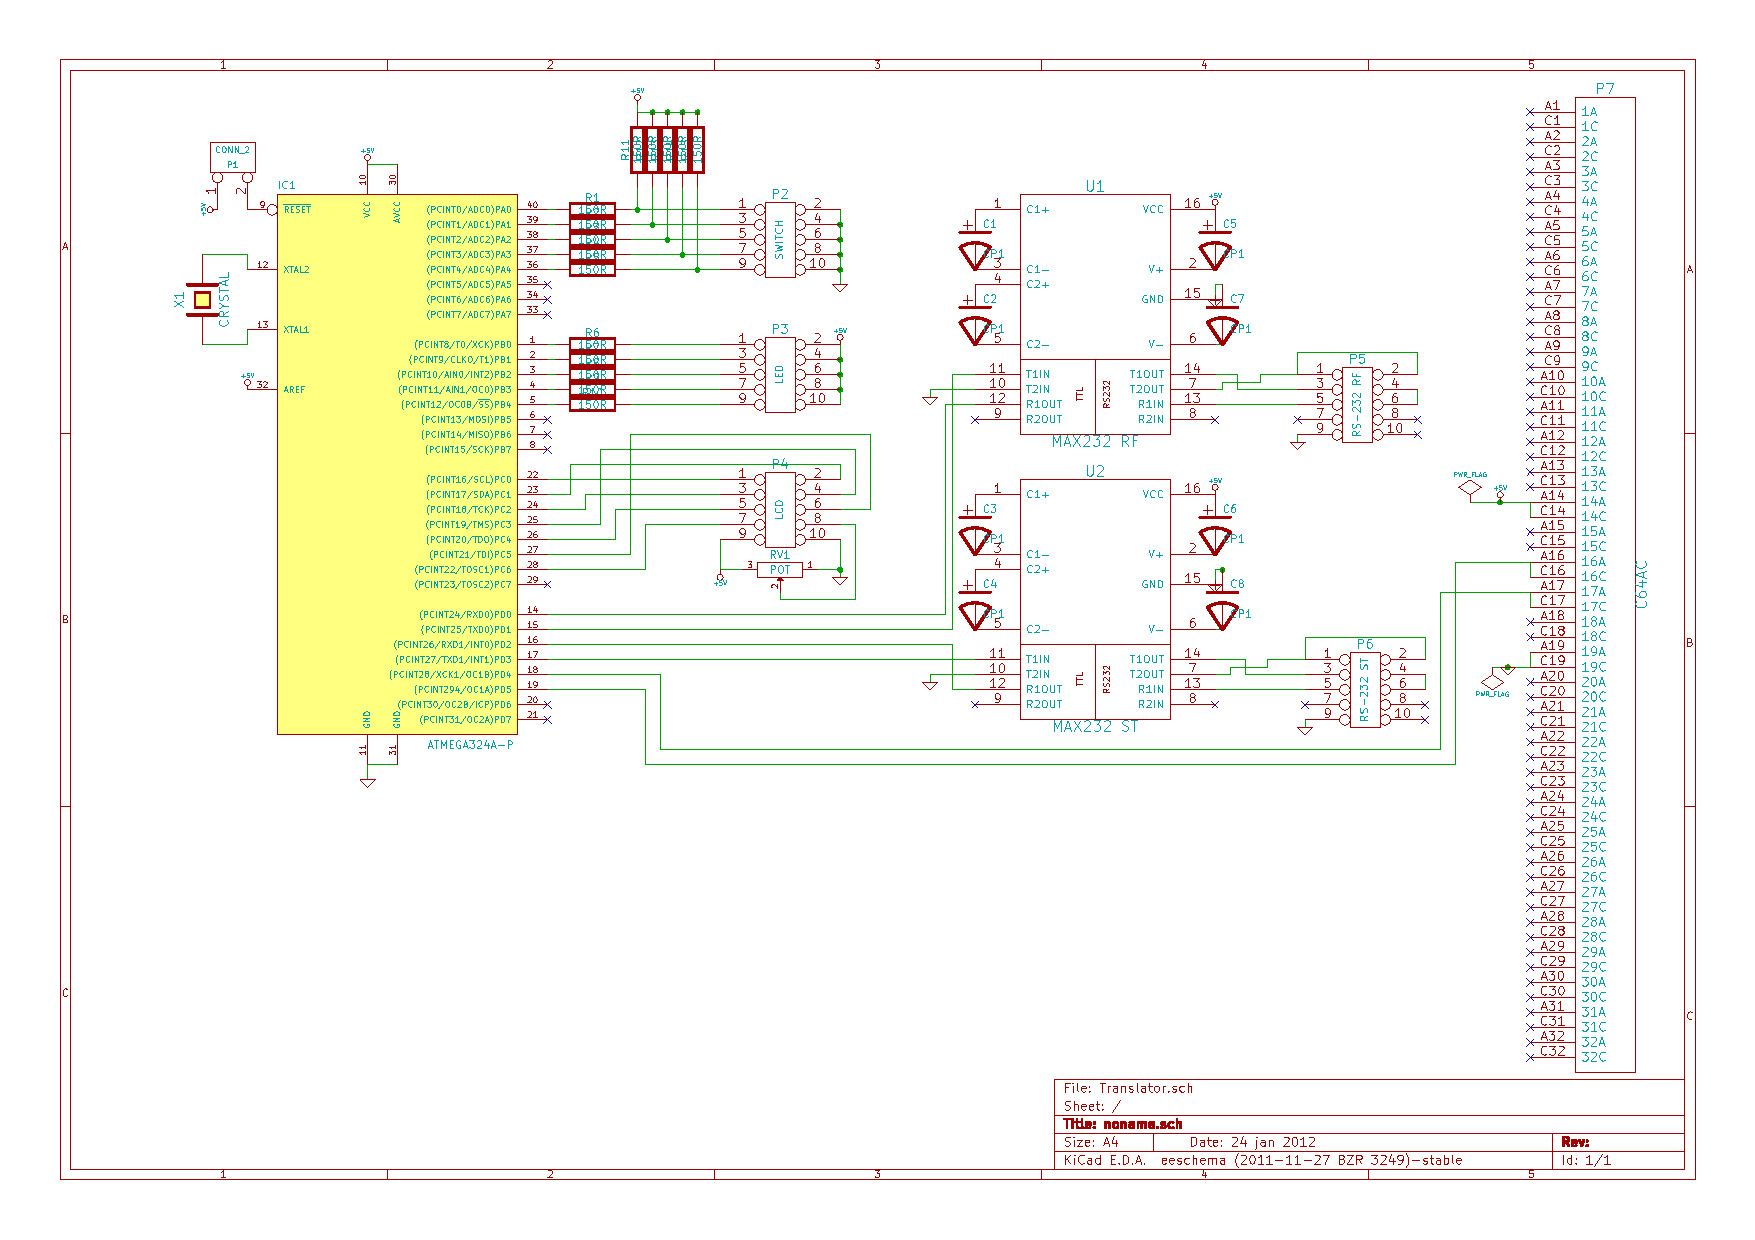
\includegraphics[width=\textwidth]{Schaltplan}
\caption{Schaltplan}
\label{fig:Schaltplan}
\end{figure}
Anschließend wird das Layout im Layouteditor entwickelt. Dabei waren mehrere enge Vorgaben einzuhalten. Da in der Werkstatt des RheinAhrCampus keine Platinen mit \Fachbegriff{Durchkontaktierungen} hergestellt werden können, sollen \Fachbegriff{Vias} vermieden, IC-Sockel, Kondensatoren und Potis nur auf der Unterseite verlötet werden. Abschließend werden die benötigten Verbindungen zwischen den Bauteilen berechnet. Die Aufgabe übernimmt im allgemeinen ein \Fachbegriff{Autorouter}. Dies kann nicht in der Software KiCad selbst durchgeführt werden. Diese Funktionalität wird jedoch durch die Java-Web-Anwendung \emph{Freeroute}[\ref{sec:V_Software}] bereitgestellt. Da der Autorouter die Aufgabe nicht zufriedenstellend lösen konnte, mussten viele Verbindungen nachträglich manuell angelegt werden. Das fertige Layout (siehe Abbildung \ref{fig:Platine}) wurde von der Werkstatt am RheinAhrCampus gefertigt und anschließend bestückt. 
\begin{figure}[h]
\centering
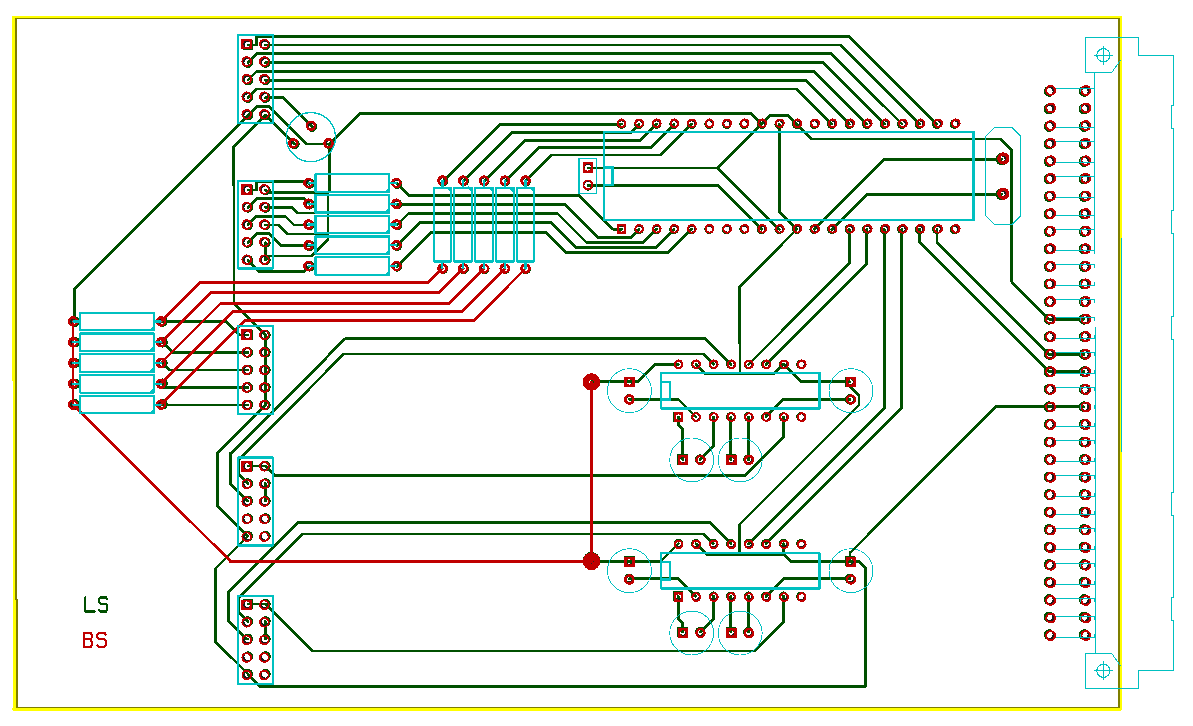
\includegraphics[width=\textwidth]{Translator_white}
\caption{Platinenlayout}
\label{fig:Platine}
\end{figure}
Über den rückwärtigen Steckverbinder wird die Platine mit der Spannungsversorgung verbunden. Zusätzlich kommen hier auch die Signale der Endschalter an. An der Vorderseite der Platine wird eine Blende verbaut. Auf dieser Blende befinden sich das LC-Display, fünf Taster, 5 LEDs und 2 serielle Schnittstellen. Alle Bauteile sind mittels Flachbandkabel, steckbar, mit der Platine verbunden.\\
Dadurch sind alle im Projekt verwendeten Komponenten auf einem 19''-Einschub (siehe Abbildung \ref{fig:Einschub}) vereint.
\begin{figure}[h]
\centering
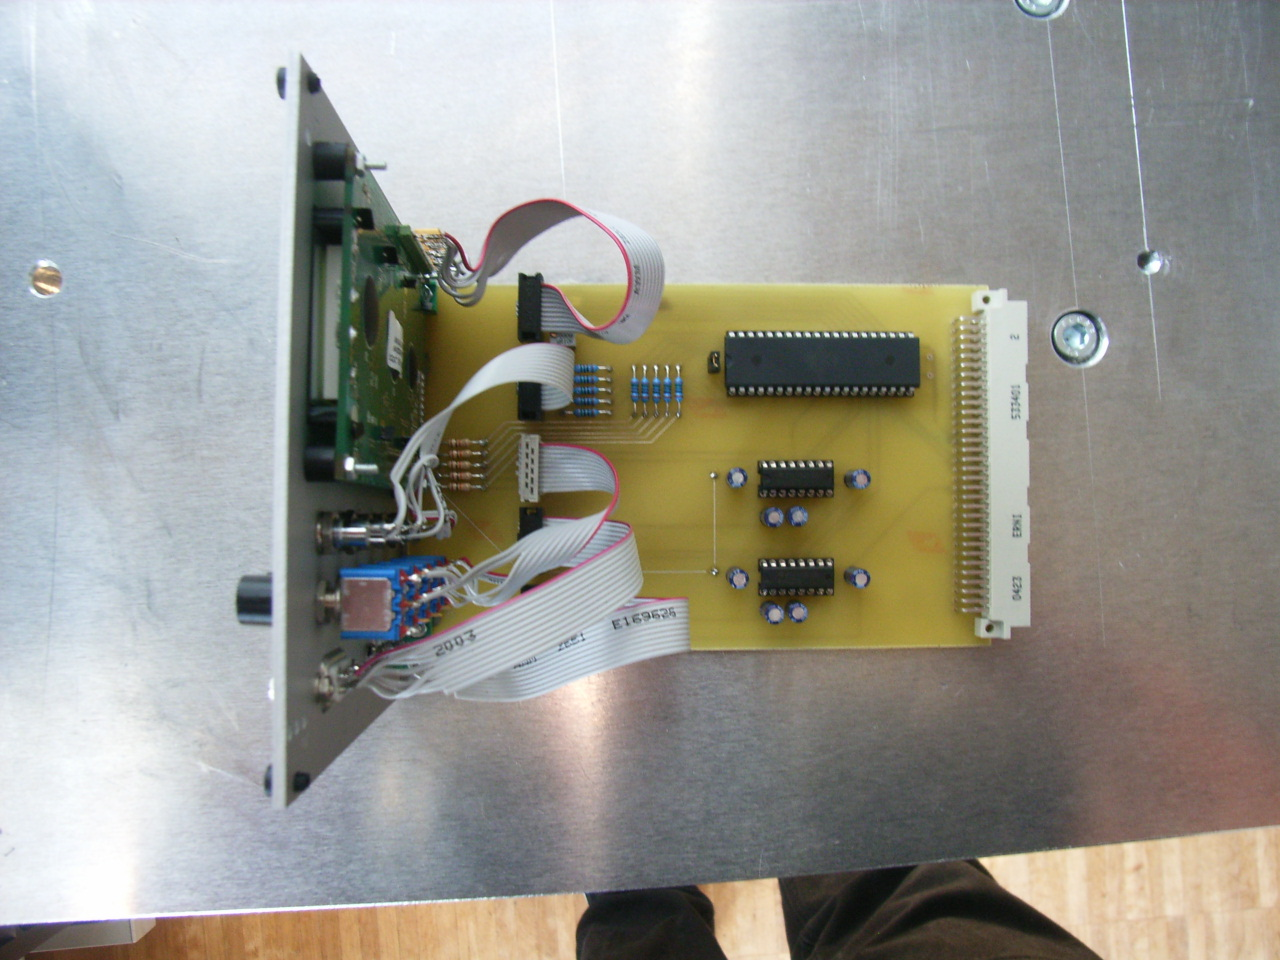
\includegraphics[width=\textwidth]{19ZollEinschub}
\caption{19''-Einschub}
\label{fig:Einschub}
\end{figure}

\chapter{Probleme und Lösungen}
\section{Entwicklungsumgebungen}
\subsection{AVR Studio 5}
\emph{AVR Studio 5}[\ref{sec:V_Software}] ist eine von Atmel bereitgestellte Entwicklungsumgebung. Diese scheint jedoch eine fehlerhafte Bibliothek zu enthalten. Die Kombination aus Mikrocontroller ATmega324A und AVR Studio 5 erzeugte nicht nachvollziehbare Probleme. Bei dem selbem Programm und einem anderem Mikrocontroller oder einer anderen Entwicklungsumgebung tauchten keine Fehler auf.
In der Entwicklungsumgebung \emph{Eclipse}[\ref{sec:V_Software}] lies sich der Fehler reproduzieren wenn der Pfad der von Atmel bereitgestellten Bibliotheken eingestellt wurde. Eine von \emph{WinAVR} bereitgestellte Bibliothek und eine selbst kompilierte \Fachbegriff{Toolchain} unter \emph{Linux} zeigten diese Probleme nicht.\\
Daher wurde zur \Fachbegriff{Open Source} Entwicklungsumgebung Eclipse mit freien Bibliotheken von WinAVR gewechselt. Dadurch wurde das Problem umgangen und das Projekt plattformunabhänig. Bis auf RapidForm2004 wurde somit nur noch freie Open Source Software verwendet.\\
\subsection{Eclipse}
Eclipse ist eine in Java programmierte freie open source Entwicklungsumgebung für Java. Sie lässt sich durch \Fachbegriff{Plugins} leicht für viele Programmiersprachen erweitern.\\
Mit dem \emph{CDT-Plugin}, dem \emph{AVR-Plugin}, der Bibliothek von \emph{WinAVR} und der Programmiersoftware \emph{AVRDude} ist Eclipse eine vollwertige Entwicklungsumgebung für Mikrocontroller von Atmel. 

\section{Interrupts}
\label{sec:Interrupts}
Viele Mikrocontroller bieten die Möglichkeit \emph{eventbasierte} \Fachbegriff{Subroutinen} auszuführen. Wenn ein sogenannter \Fachbegriff{Interrupt} ausgelöst wird, wird das Hauptprogramm unterbrochen und eine entsprechende \Fachbegriff{Interrupt-Service-Routine}, kurz ISR, ausgeführt. Nach Beendigung der ISR wird das Hauptprogramm an der Stelle wieder aufgenommen, an der es unterbrochen wurde. ISR dürfen nur sehr wenige Befehle enthalten und sollten innerhalb weniger \Fachbegriff{Taktzyklen} abgeschlossen sein.\\
Interrupts können z.B. der Überlauf eines internen Timer, oder ein externens Signal an einem Pin sein. Im Projekt werden Externe-Interrupts für die Endschalter, Timer-Überlauf-Interrupts für das Entprellen der Taster und der Watchdog-Interrupt zum erkennen von Fehlern genutzt. 
\subsection{Endschalter}
\label{sec:Endschalter_SW}
Die Endschalter sind über die Schrittmotorkarten und eine Brücke auf der Rückseite der Einschubsteckplätze mit der Mikrocontrollerplatine verbunden. Dort sind sie an 2 Interrupt Pins angeschlossen. Bei einem Flankenwechsel an den Pins wird ein Interrupt ausgelöst. \\
Mit den Zeilen 1--2 des Codelistings \ref{lst:ISR_ES} werden Pin-Change-Interrupts für bestimmte Pins zugelassen. Die Zeilen 3--7 und 8--12 zeigen die Interrupt-Service-Routinen für die beiden Interrupts.
\lstset{language=C, basicstyle=\footnotesize, showstringspaces=false, tabsize=2}
\lstinputlisting[label=lst:ISR_ES,caption=ISR: Endschalter]{Code/ISR_Endschalter.c}
\subsection{Watchdog}
Der \Fachbegriff{Watchdog} ist eine Sicherungseinrichtung des Mikrocontroller. In regelmäßigen Abständen wird überprüft ob das Watchdog-Bit gesetzt ist und anschließend zurück gesetzt. Das Bit muss innerhalb der voreingestellten Zeit immer wieder neu gesetzt werden. Dies kann mit der Funktion \Code{wdt\_reset()} realisiert werden. Ist das Bit nicht gesetzt, wird der Mikrocontroller zurückgesetzt. Dies geschieht z.B. bei ungewollten Endlosschleifen.\\
Mit den Zeilen 3--10 des Codelisting \ref{lst:Watchdog} wird der Watchdog initialisiert und festgelegt in welchen Zeitintervallen das Watchdog-Bit überprüft werden soll. Der Ablauf zum einstellen des Zeitinveralls muss genau wie im Datenblatt des Mikrocontroller beschrieben eingehalten werden. Dies verhindert ein versehentliches Ändern der Einstellung. 
Ist das Fusebit \emph{WDTON} gesetzt kann der Watchdog nicht abgeschaltet werden (siehe Kapitel \ref{sec:Fuses}).\\
Wahlweise kann kurz vor dem zurücksetzen des Mikrocontroller noch die Watchdog-ISR durchlaufen werden. Im Projekt wird in der ISR die \emph{Fehler-LED} eingeschaltet und eine Meldung auf dem LC-Display ausgegeben (siehe Codelisting \ref{lst:Watchdog} Zeilen 12-16).
\lstset{language=C, basicstyle=\footnotesize, showstringspaces=false, tabsize=4}
\lstinputlisting[label=lst:Watchdog,caption=Watchdog]{Code/Watchdog.txt}

\section{Fuses}
\label{sec:Fuses}
Als \Fachbegriff{Fuses} werden Register bezeichnet mit denen sich, auf Hardwareebene, das Verhalten des Mikrocontrollers verändern lässt. Im Projekt wurden folgende Fuses problematisch.
\begin{itemize}
\item \textbf{JTAGEN} - Ist dieses Bit gesetzt, kann an 4 Pins des \emph{PortB} ein \Fachbegriff{JTAG-Debugger} angeschlossen werden. Debuggen auf Hardwareebene bietet viele Vorteile. Diese wurden im Projekt jedoch nicht genutzt, da kein JTAG-Debugger zur Verfügung stand und PortB für die LEDs genutzt wurde.
\item \textbf{WDTON} - Ist dieses Bit gesetzt, läuft der Watchdog-Timer immer mit. Wird der Watchdog dann nicht regelmäßig mit der Funktion \Code{wdt\_reset()} zurückgesetzt, startet der Mikrocontroller ständig neu. 
\item \textbf{CKDIV8} - Teilt den Systemtakt des Mikrocontroller durch 8. Dies ist Energiesparender. Der geringere Takt muss in F\_CPU angepasst werden da sonst zeitkritische Prozesse mit der falschen Geschwindigkeit ablaufen. Das Bit wurde jedoch im Projekt nicht gesetzt.
\item \textbf{CKOUT} - An einem Pin an \emph{PortB} wird der Systemtakt ausgegeben. Dieser kann dann leicht mit einem Frequenz-Messgerät überprüft werden. Der Pin kann dann jedoch nicht anderweitig genutzt werden.
\item \textbf{CKSELX} - Über diese 4 Bits kann der Systemtakt eingestellt werden.
\end{itemize}
\begin{longtable}{|l|l|} 
\caption{Fuses}\\
\hline
\label{tab:Fuses}OCDEN & On Chip Debugging\\ \hline 
JTAGEN & Hardware Debugging\\ \hline 
SPIEN & Serial Program and Data Downloading\\ \hline 
WDTON & Watchdog Timer always on\\ \hline 
EESAVE & EEPROM memory is preserved through the Chip Erase\\ \hline 
BOOTSZ1 & Select Boot Size\\ \hline 
BOOTSZ0 & Select Boot Size\\ \hline 
BOOTRST & Select Reset Vector\\ \hline 
CKDIV8 & Divide clock by 8\\ \hline 
CKOUT & Clock output\\ \hline 
SUT1 & Select start-up time\\ \hline 
SUT0 & Select start-up time\\ \hline 
CKSEL3 & Select Clock source\\ \hline 
CKSEL2 & Select Clock source\\ \hline 
CKSEL1 & Select Clock source\\ \hline 
CKSEL0 & Select Clock source\\ \hline 
\end{longtable} 
